\documentclass{beamer}

\newcommand{\course}{CS 1331 Introduction to Object Oriented Programming}
\newcommand{\lesson}{Review 3: Exceptions, Recursion, and Swing}
\newcommand{\code}{http://www.cc.gatech.edu/~simpkins/teaching/gatech/cs1331/code}

\author[Chris Simpkins] 
{Christopher Simpkins \\\texttt{chris.simpkins@gatech.edu}}
\institute[Georgia Tech] % (optional, but mostly needed)

\date[CS 1331]{}

\subject{\lesson}


% If you have a file called "university-logo-filename.xxx", where xxx
% is a graphic format that can be processed by latex or pdflatex,
% resp., then you can add a logo as follows:

% \pgfdeclareimage[width=0.6in]{coc-logo}{cc_2012_logo}
% \logo{\pgfuseimage{coc-logo}}

\mode<presentation>
{
  \usetheme{Berlin}
  \useoutertheme{infolines}

  % or ...

 \setbeamercovered{transparent}
  % or whatever (possibly just delete it)
}

\usepackage{hyperref}
\usepackage{fancybox}
\usepackage{listings}
\usepackage[abbr]{harvard}

\usepackage[english]{babel}
% or whatever

\usepackage[utf8]{inputenc}
% or whatever

\usepackage{times}
\usepackage[T1]{fontenc}
% Or whatever. Note that the encoding and the font should match. If T1
% does not look nice, try deleting the line with the fontenc.


\usepackage{listings}
 
% "define" Scala
\lstdefinelanguage{scala}{
  morekeywords={abstract,case,catch,class,def,%
    do,else,extends,false,final,finally,%
    for,if,implicit,import,match,mixin,%
    new,null,object,override,package,%
    private,protected,requires,return,sealed,%
    super,this,throw,trait,true,try,%
    type,val,var,while,with,yield},
  otherkeywords={=>,<-,<\%,<:,>:,\#,@},
  sensitive=true,
  morecomment=[l]{//},
  morecomment=[n]{/*}{*/},
  morestring=[b]",
  morestring=[b]',
  morestring=[b]""",
}

\usepackage{color}
\definecolor{dkgreen}{rgb}{0,0.6,0}
\definecolor{gray}{rgb}{0.5,0.5,0.5}
\definecolor{mauve}{rgb}{0.58,0,0.82}
 
% Default settings for code listings
\lstset{frame=tb,
  language=scala,
  aboveskip=2mm,
  belowskip=2mm,
  showstringspaces=false,
  columns=flexible,
  basicstyle={\scriptsize\ttfamily},
  numbers=none,
  numberstyle=\tiny\color{gray},
  keywordstyle=\color{blue},
  commentstyle=\color{dkgreen},
  stringstyle=\color{mauve},
  frame=single,
  breaklines=true,
  breakatwhitespace=true,
  keepspaces=true
  %tabsize=3
}


\title[\course] % (optional, use only with long
                                      % paper titles)
{\lesson}

\subtitle{}
%% {Include Only If Paper Has a Subtitle}

\newcommand{\link}[2]{\href{#1}{\textcolor{blue}{\underline{#2}}}}


% If you wish to uncover everything in a step-wise fashion, uncomment
% the following command: 

% \beamerdefaultoverlayspecification{<+->}


\begin{document}

\begin{frame}
  \titlepage
\end{frame}

%------------------------------------------------------------------------
\begin{frame}[fragile]{Exam 3 Topics}


\begin{itemize}
\item Exceptions
\item Recursion
\item Swing
\end{itemize}


\end{frame}
%------------------------------------------------------------------------

%------------------------------------------------------------------------
\begin{frame}[fragile]{Exceptions}

\begin{itemize}
\item How they work
\item Checked and unchecked exceptions
\item The ``declare or throw'' rule
\item Multiple catch blocks
\end{itemize}


\end{frame}
%------------------------------------------------------------------------

%------------------------------------------------------------------------
\begin{frame}[fragile]{Throwing Exceptions is a Control Flow Mechanism}


What does this code print?
\begin{lstlisting}[language=Java]
public class Wee {

    static void bar() throws Throwable {
        throw new Throwable("Wee!");
    }

    static void foo() throws Throwable {
        bar();
        System.out.println("Foo!");
    }

    public static void main(String[] args) {
        try {        
            foo();
        } catch (Throwable t) {
            System.out.println(t.getMessage());
        }
        System.out.println("I'm still running.");
    }
}
\end{lstlisting}

\end{frame}
%------------------------------------------------------------------------

%------------------------------------------------------------------------
\begin{frame}[fragile]{Java's Exception Hierarchy}

\begin{columns}[t]
\begin{column}{2in}
\begin{center}
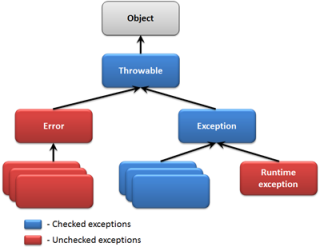
\includegraphics[height=2.5in]{hierarchy_of_java_exceptions.png}
\end{center}
\end{column}
\begin{column}{3in}
\begin{itemize}
\item Most (checked) exceptions will subclass {\tt Exception}
\item Most uncheked exceptions will subclass {\tt RuntimeException}
\item {\tt Error} is for compiler hackers.  Don't use it directly.
\end{itemize}
\end{column}
\end{columns}

\end{frame}
%------------------------------------------------------------------------

%------------------------------------------------------------------------
\begin{frame}[fragile]{Catch or Declare}


The method {\tt initFromFile} throws {\tt FileNotFoundException}. Since {\tt FileNotFoundException} is a checked exception, you must deal with it in one of two ways:\\
\vspace{.1in}
{\it catch}:
\vspace{-.05in}
\begin{lstlisting}[language=Java,escapechar=`]
public void myMethod(String dataFile) {
    try {
        initFromFile(new File(dataFile));
    } `\colorbox{yellow}{catch (FileNotFoundException e) \{}`
        System.out.println(e.getMessage());
    }
}
\end{lstlisting}
or {\it declare}:
\vspace{-.05in}
\begin{lstlisting}[language=Java,escapechar=`]
public void myMethod(String dataFile) `\colorbox{yellow}{throws FileNotFoundException \{}`
      initFromFile(new File(dataFile));
}
\end{lstlisting}



\end{frame}
%------------------------------------------------------------------------

%------------------------------------------------------------------------
\begin{frame}[fragile]{Multiple Catch Blocks}


What's wrong with this code?
\begin{lstlisting}[language=Java]
public class Company {
    private ArrayList<Employee> employees;

    public Company(String employeeDataFile) {
        employees = new ArrayList<Employee>(10);
        try {
            initFromFile(new File(employeeDataFile));
        } catch (Exception e) {
            System.out.println("Exception occurred: "+e.getMessage());
        } catch (FileNotFoundException e) {
            System.out.println("Employee data file not found.");
        } catch (ParseException e) {
            System.out.println("Malformed data file: "+e.getMessage();
        }
    }
    //...
}
\end{lstlisting}

\end{frame}
%------------------------------------------------------------------------

%------------------------------------------------------------------------
\begin{frame}[fragile]{Multiple Catch Blocks}


The first catch clause will always be the one executed, because {\tt Exception} is a superclass of {\tt FileNotFoundException} and {\tt ParseException}.
\begin{lstlisting}[language=Java,escapechar=`]
public class Company {
    private ArrayList<Employee> employees;

    public Company(String employeeDataFile) {
        employees = new ArrayList<Employee>(10);
        try {
            initFromFile(new File(employeeDataFile));
        } catch (`\colorbox{yellow}{Exception e}`) {
            System.out.println("Exception occurred: "+e.getMessage());
        } catch (FileNotFoundException e) {
            System.out.println("Employee data file not found.");
        } catch (ParseException e) {
            System.out.println("Malformed data file: "+e.getMessage();
        }
    }
    //...
}

\end{lstlisting}

\end{frame}
%------------------------------------------------------------------------

%------------------------------------------------------------------------
\begin{frame}[fragile]{Recursion}


\begin{itemize}
\item A recursive processes or data structure is defined in terms of itself
\item A properly written recursive function must
\begin{itemize}
\item hand the base case, and
\item convergence to the base case.
\end{itemize}
\item Failure to properly handle the base case or converge to the base (divergence) case may result in infinite recursion.
\end{itemize}


\end{frame}
%------------------------------------------------------------------------

%------------------------------------------------------------------------
\begin{frame}[fragile]{A Recursive Factorial Function}


Point out the base case and explain how this function converges to it.
\vspace{-.05in}
\begin{lstlisting}[language=Java]
public static int fac(int n) {
    if (n <= 1) {
        return 1;
    } else {
        return n * fac(n - 1);
    }
}
\end{lstlisting}
\vspace{-.05in}
The substitution model of evaluation is a tool for understanding recursive processes.  Here's {\tt fac(5)}:
\vspace{-.05in}
\begin{lstlisting}[language=Java]
fac(5)
5 * fac(4)
5 * 4 * fac(3)
5 * 4 * 3 * fac(2)
5 * 4 * 3 * 2 * fac(1)
5 * 4 * 3 * 2 * 1
5 * 4 * 3 * 2
5 * 4 * 6
5 * 24
120
\end{lstlisting}


\end{frame}
%------------------------------------------------------------------------


%------------------------------------------------------------------------
\begin{frame}[fragile]{Swing}


Lots of stuff in Swing.  A few highlights:
\begin{itemize}
\item Components with {\tt ActionListener}s
\item Use {\tt private} inner classes (not anonymous inner classes)
\item Avoid using a single monolithic class and identifying the event firer with {\tt getActionCommand()}
\end{itemize}


\end{frame}
%------------------------------------------------------------------------

%------------------------------------------------------------------------
\begin{frame}[fragile]{The Wrong Way to Write an {\tt ActionListener}}


\begin{lstlisting}[language=Java,escapechar=`]
public class BadListener extends JFrame `\colorbox{yellow}{implements ActionListener}` {

    public BadListener() {
        super("Bad");
        setDefaultCloseOperation(EXIT_ON_CLOSE);
        JButton helloButton = new JButton("Hello");
        helloButton.addActionListener(this);
        JButton goodByeButton = new JButton("Good bye");
        goodByeButton.addActionListener(this);
        add(helloButton, BorderLayout.NORTH);
        add(goodByeButton, BorderLayout.SOUTH);
    }

    public void actionPerformed(ActionEvent e) {
        String button = `\colorbox{yellow}{e.getActionCommand()}`;
        if (button.equals("Hello")) {
            System.out.println("Hello was perssed.");
        } else if (button.equals("Good bye")) {
            System.out.println("Good bye was perssed.");
        }
    }
}
\end{lstlisting}

\end{frame}
%------------------------------------------------------------------------

%------------------------------------------------------------------------
\begin{frame}[fragile]{A Better Way to Write an {\tt ActionListener}}

\vspace{-.1in}
\begin{lstlisting}[language=Java]
public class BetterListener extends JFrame {

    private class HelloListener implements ActionListener {
        public void actionPerformed(ActionEvent e) {
            System.out.println("Hello was pressed.");
        }
    }
    private class GoodByeListener implements ActionListener {
        public void actionPerformed(ActionEvent e) {
            System.out.println("Good bye was pressed.");
        }
    }
    public BetterListener() {
        super("Better Listener");
        setDefaultCloseOperation(EXIT_ON_CLOSE);
        JButton helloButton = new JButton("Hello");
        helloButton.addActionListener(new HelloListener());
        JButton goodByeButton = new JButton("Good bye");
        goodByeButton.addActionListener(new GoodByeListener());
        add(helloButton, BorderLayout.NORTH);
        add(goodByeButton, BorderLayout.SOUTH);
    }
}
\end{lstlisting}


\end{frame}
%------------------------------------------------------------------------

% %------------------------------------------------------------------------
% \begin{frame}[fragile]{}


% \begin{lstlisting}[language=Java]

% \end{lstlisting}

% \begin{itemize}
% \item
% \end{itemize}


% \end{frame}
% %------------------------------------------------------------------------


\end{document}
